%%%%%%%%%%%%%%%%%%%%%%%%%%%%%%%%%%%%%%%%%%%%%%%%%%%%%%%%%%%%
\section{Introduction}
%\subsection{Neutrinoless double beta decay.}
Neutrinos, unlike the other fermions of the Standard Model of particle physics, could be Majorana particles, that is, indistinguishable from their antiparticles. The existence of Majorana neutrinos would have profound implications in particle physics and cosmology. 

 If neutrinos are Majorana particles, there must exist a new scale of physics (at a level inversely proportional to the neutrino masses) that characterises the underlying dynamics beyond the Standard Model. The existence of such a new scale provides the simplest explanation of why neutrino masses are so much lighter than the charged fermions. Indeed, understanding the new physics responsible for neutrino masses is one of the most important open questions in particle physics, and could have profound implications in our comprehension of the mechanism of symmetry breaking, the origin of mass and the flavour problem. 

The discovery of Majorana neutrinos would also mean that total lepton number is not conserved, an observation that could be linked to the origin of the matter-antimatter asymmetry observed in the Universe today. This is because the new physics responsible for neutrino masses could provide a new mechanism to generate this asymmetry, via a process called leptogenesis. Although the predictions are model dependent, two essential ingredients must be confirmed experimentally for leptogenesis to occur: 1) the violation of lepton number and 2) CP violation in the lepton sector. 

The only practical way to establish experimentally whether neutrinos are their own antiparticles, and whether lepton number is not conserved, is the detection of neutrinoless double beta decay (\bbonu). This is a hypothetical, very slow nuclear transition in which a nucleus with $Z$ protons decays into a nucleus with $Z+2$ protons and the same mass number $A$, emitting two electrons that carry essentially all the energy released (\Qbb). The process can occur if and only if neutrinos are Majorana particles. 

%%%%%%%%%%%%%%%%%%%%%%%%%%%%%%%%%%%%%%%%%%%%%%%%%%%%%%%%%%%%
\subsection{The experimental landscape}
The detectors used in double beta decay searches are designed to measure the energy of the radiation emitted by a \bb\ source. In the case of \bbonu, the sum of the kinetic energies of the two released electrons is fixed by the mass difference between the parent and the daughter nuclei: $Q_{\bb} \equiv M(Z,A)-M(Z+2,A)$. However, due to the finite energy resolution of any detector, \bbonu\ events are reconstructed within an energy region centered around \Qbb, typically following a gaussian distribution (Region of Interest, or ROI). Other processes occurring in the detector can fall in the ROI, becoming a background and compromising drastically the expected sensitivity. It follows that \bbonu\ experiments require {\bf excellent energy resolution}, and indeed the field has been traditionally dominated by germanium calorimeters, devices with superb resolution.

All double beta decay experiments have to deal with an intrinsic background, the \bbtnu, the standard process of a double $\beta$-decay with the emission of two neutrinos, that can only be suppressed by means of good energy resolution. Backgrounds of cosmogenic origin force the {\bf underground operation of the detectors}. Natural radioactivity emanating from the detector materials and surroundings can easily overwhelm the signal peak, and hence {\bf careful selection of radiopure materials is also essential}. {\bf Additional experimental signatures} that allow the distinction between signal and background are certainly a bonus, and this has been in the last few years an important line of work to increase the sensitivity of \bbonu\ detectors. Several other factors such as {\bf detection efficiency} or the {\bf scalability to large masses} must also be taken into account during the design of a double beta decay experiment.
 
 \subsection{Recent results}
 Three new-generation experiments, with fiducial masses in the range of 100~kg, have recently published the results of their searches for \bbonu\ processes. These are: GERDA, a high resolution calorimeter based on \GE\ diodes; KamLAND-Zen, a low resolution, high-mass, self-shielding liquid scintillator calorimeter, with xenon dissolved in the scintillator; and EXO-200, a liquid xenon (LXe) TPC. All the experiments published null results and therefore a lower limit on the period of \bbonu\ processes, \Tonu. This lower limit can be translated into an upper limit on the \emph{effective Majorana mass} of the electron neutrino defined as:
\begin{equation}
\mbb = \Big| \sum_{i} U^{2}_{ei} \ m_{i} \Big| \, ,
\end{equation}
%
where $m_{i}$ are the neutrino mass eigenstates and $U_{ei}$ are elements of the neutrino mixing matrix. The mass \mbb\ is related to the period through the equation:

\begin{equation}
(T^{0\nu}_{1/2})^{-1} = G^{0\nu} \ \big|M^{0\nu}\big|^{2} \ \mbb^{2} \, .
\label{eq:Tonu}
\end{equation}

In Eq.~\ref{eq:Tonu}, $G^{0\nu}$ is an exactly-calculable phase-space integral for the emission of two electrons and $M^{0\nu}$ is the nuclear matrix element (NME) of the transition, which has to be evaluated theoretically. The uncertainty in the NME affects the value of \mbb\ which can be obtained from \Tonu.
 
{\bf GERDA} \footcite{Agostini:2013mzu} has a resolution of $\sim$0.2 \% FWHM around the \Qbb\ of \GE. The specific background rate in the ROI is $10^{-2}$ \ckky\ and the total exposure deployed is 21.6 kg$\cdot$yr. The experiment sets a limit $\Tonu(\GE)> 2 \times 10^{25}$~yr, which translates into an upper limit range for \mbb\ of $[258-649]$~milli electronvolts (meV). The lowest value of the \mbb\ upper limit corresponds to the IBM2 NME set\footcite{Barea:2013bz}, while the highest value corresponds to the ISM set\footcite{Menendez:2008jp}.

{\bf EXO} \footcite{Albert:2014awa} achieves an energy resolution of 3.6\% FWHM at \Qbb, and a background rate of $ 4 \times 10^{-3}\ckky$. The total exposure used for the published result is 100 kg$\cdot$~yr. The EXO Collaboration has published a limit on the half-life of \bbonu\ in \XE\ of $T_{1/2}^{0\nu}(\XE) > 2 \times 10^{25}$~yr. The limit translates into an upper limit range for \mbb\ of $[125-352]$~meV, depending on the NME.

{\bf KamLAND-Zen} \footcite{TheKamLAND-Zen:2014lma} compensates a worse energy resolution of 10\% FWHM at \Qbb\ with a very small background rate of $\sim 4 \times 10^{-4}$ \ckky. After an exposure of 108.8 kg$\cdot$~yr, they obtain a limit  $T_{1/2}^{0\nu}(\XE) > 2.6 \times 10^{25}$~yr, which translates into an upper limit range for \mbb\ of $[110-309]$~meV, depending on the NME.

 \subsection{Potential for discovery}
 
 %%%%%%
\begin{figure}
\centering
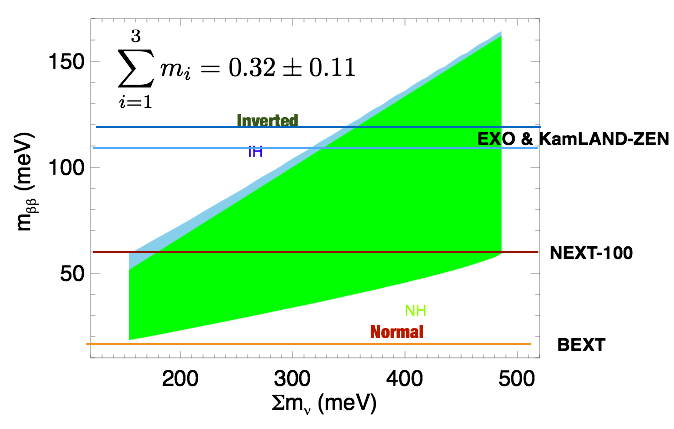
\includegraphics[width=0.70\textwidth]{img/SensiCRR.png}
\caption{\small The allowed \mbb\ region (68\% CL for two degrees of freedom), as a function of the sum of the neutrino masses, assuming that 
$\sum m_i = 0.32\pm 0.11$~eV. The blue lines mark the sensitivity of EXO and KamLAND-ZEN, the xenon-based detectors currently leading the field. The red line shows the sensitivity of NEXT after 3 years operation, which gives the experiment a sizable chance of making a discovery.} 
\label{fig.mbb}
\end{figure}
%%%%%%

 Several analyses from recent cosmological results suggest that the sum of the masses of the three neutrinos could be $\sim$ 0.3 eV\footcite{PhysRevLett.112.051303}. G\'omez-Cadenas and collaborators have demonstrated that, in this case, if the neutrino is a Majorana particle, then, $\mbb \sim [20-150]$~ meV \footcite{GomezCadenas:2013ue}, as shown in Figure \ref{fig.mbb}. In this scenario, the sensitivity of GERDA is outside the ``cosmologically relevant region'' (CRR), while both EXO-200 and KamLAND-Zen would have already explored a significant fraction of CRR {\em for the most optimistic NME set} (while they would be outside CRR for the most pessimistic). 
 
Clearly, the experimental effort to determine if the neutrino is a Majorana particle, far from being completed is, rather, in its infancy. To establish unambiguously that the neutrino is (or not) a Majorana particle, even in this favourable scenario in which the sum of the neutrino masses is relatively high, experiments must be sensitive to $\mbb \sim 20$~meV, {\em even for the most pessimistic NME} set. This is a major challenge.
% 
 
%%%%%%%%%%%%%%%%%%%%%%%%%%%%%%%%%%%%%%%%%%%%%%%%%%%%%%%%%%%%
\section{The NEXT experiment and its innovative concepts}
\begin{figure}
\centering
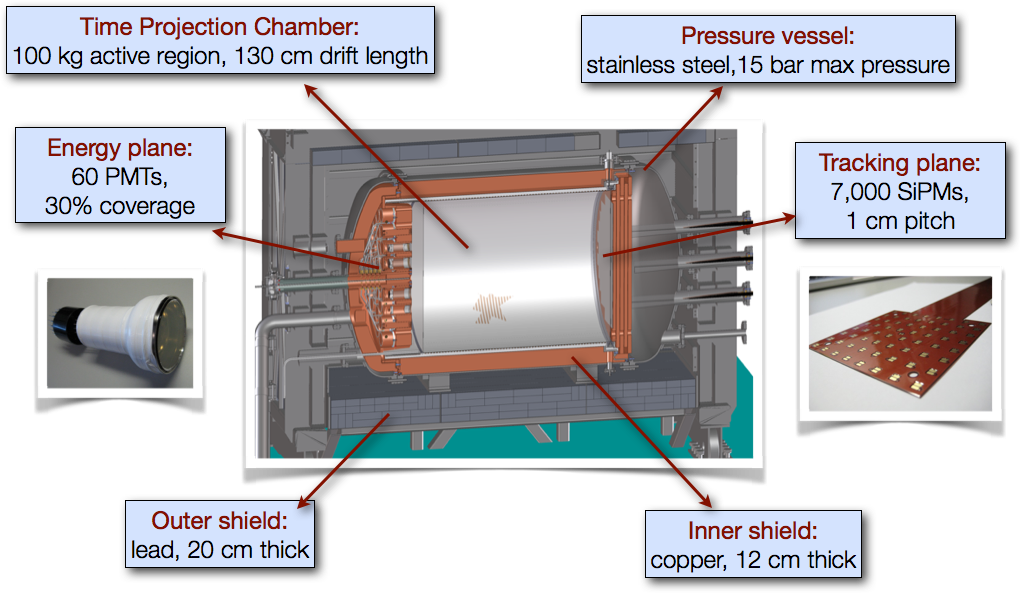
\includegraphics[width=0.9\textwidth]{img/NEXT.png}
\caption{\small A drawing of the NEXT-100 detector showing its main parts. The pressure vessel (PV) is made of a radio pure steel-titanium alloy. The PV dimensions are 130~cm inner diameter, 222~cm length, 1~cm thick walls, fot a total mass of 1\,200 kg. The inner copper shield (ICS) is made of ultra-pure copper bars and is 12~cm thick, with a total mass of 9\,000 kg. The time projection chamber includes the field cage, cathode, EL grids and HV penetrators.
The light tube is made of thin teflon sheets coated with TPB (a wavelength shifter). 
The energy plane is made of 60 PMTs housed in copper enclosures (cans).
The tracking plane is made of MPPCs arranged into dice boards (DB). 
} \label{fig.NEXT100}
\end{figure}

The \emph{Neutrino Experiment with a Xenon TPC} (NEXT)\footcite{next} will search for \bbonu\ in \XE\ using  high-pressure xenon gas  time projection chambers (\HPXE). The advantages of the technology are: 
a) {\bf excellent energy resolution}, with an intrinsic limit of about 0.3\% FWHM at \Qbb, close to that of \GE\ detectors; b)
{\bf tracking capabilities} that provide a powerful topological signature to discriminate between signal (two electron tracks with a common vertex) and background (mostly, single electrons); c)
{\bf a fully active and homogeneous detector}, with no dead regions; d) {\bf scalability} of the technique to large masses; e) the possibility of exciting the barium ion produced in the xenon decay from the fundamental state \TwoS\ to the state \TwoP, using a ``blue'' laser (493.54 nm), and observing the ``red light'' emitted in the transition from \TwoP\ to \TwoD, thus ``tagging'' the presence of a barium atom in the xenon gas, which cannot be produced by any known background. 

The design of the NEXT-100 detector (Figure \ref{fig.NEXT100}) is optimised for energy resolution by using proportional electroluminescent (EL) amplification of the ionisation signal. The detection process involves the use of the prompt scintillation light from the gas as start-of-event time, and the drift of the ionisation charge to the anode by means of an electric field ($\sim0.3$ kV/cm at 15 bar) where secondary EL scintillation is produced in the region defined by two highly transparent meshes, between which there is a field of $\sim20$ kV/cm at 15 bar. The detection of EL light provides an energy measurement using photomultipliers (PMTs) located behind the cathode (the \emph{energy plane}) as well as tracking through its detection a few mm away from production at the anode, via a dense array of silicon photomultipliers (the \emph{tracking plane}).

\subsection{NEXT prototypes}

\begin{figure}
\centering
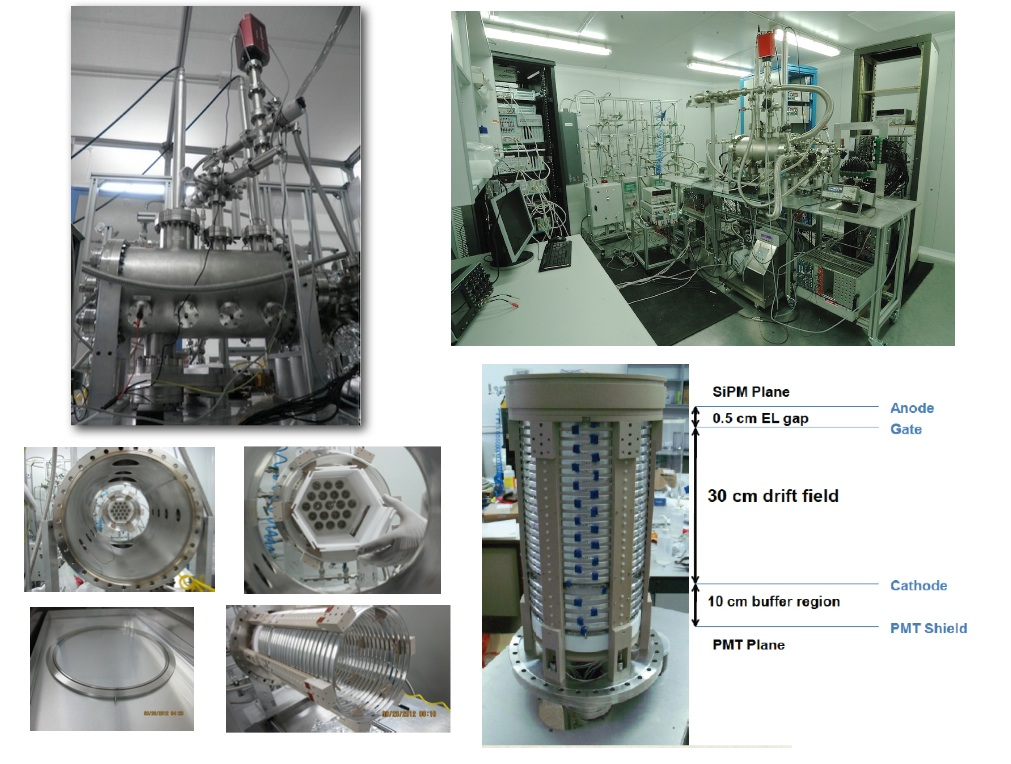
\includegraphics[width=0.99\textwidth]{img/DemoSetup2.jpg}
\caption{\small The NEXT-DEMO prototype. Top-left: the pressure vessel, showing the HVFT and the mass spectrometer; bottom-left: an expanded view of the detector; (c) Teflon light tube; (d) energy plane, made of pressure resistant Hamamatsu R7378A PMTs; (e) field cage; (f) tracking plane equipped with 300 Hamamatsu MPPCs; top-right: the full setup at IFIC; bottom right: the field cage.} \label{fig.DEMO}
\end{figure}
%%%%%%%%%%

\begin{figure}
\centering
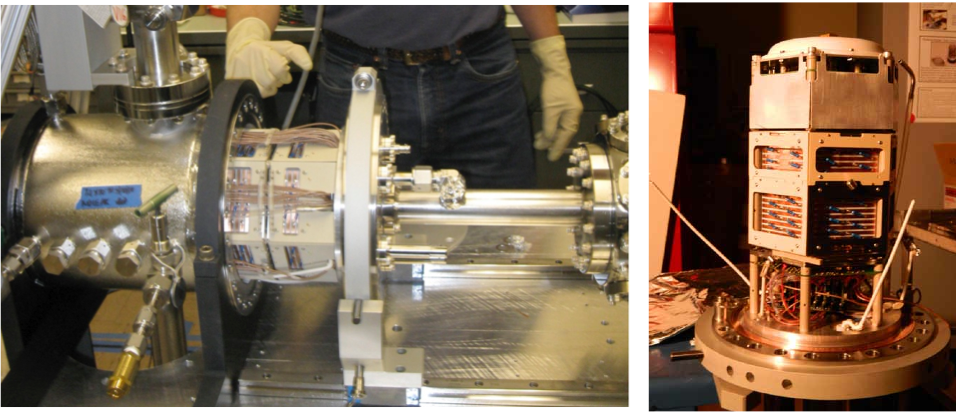
\includegraphics[width=0.99\textwidth]{img/DBDM.png}
\caption{\small The NEXT-DBDM prototype. Top-left: the pressure vessel, in the moment in which the field cage is inserted; (b) the field cage.} \label{fig.DBDM}
\end{figure}


NEXT-DEMO, shown in figure \ref{fig.DEMO}, is as a large-scale prototype of NEXT-100. The pressure vessel has a length of 60 cm and a diameter of 30 cm. The vessel can withstand a pressure of up to 15 bar and hosts typically 1-2 kg of xenon. NEXT-DEMO is  equipped with an energy plane made of 19 Hamamatsu R7378A PMTs and a tracking plane made of 256 Hamamatsu SiPMs. 

The detector has been operating successfully for more than two years and has demonstrated: (a) very good operational stability, with no leaks and very few sparks; (b) good energy resolution ; (c) track reconstruction with PMTs and with SiPMs coated with TPB; (d) excellent electron drift lifetime, of the order of 20 ms.Its construction, commissioning and operation has been instrumental in the development of the required knowledge to design and build the NEXT detector.

The NEXT-DBDM prototype (Figure \ref{fig.DBDM}) is a smaller chamber, with only 8 cm drift, but an aspect ratio (ratio diameter to length) similar to that of NEXT-100. The device has been used to perform detailed energy resolution studies, as well as studies to characterise neutrons in an \HPXE. NEXT-DBDM achieves a resolution of 1\% FWHM at 660 keV and 15 bar, which extrapolates to 0.5\% at \Qbb.

\subsection{Topological signature}

%%%%%
\begin{figure}
\centering
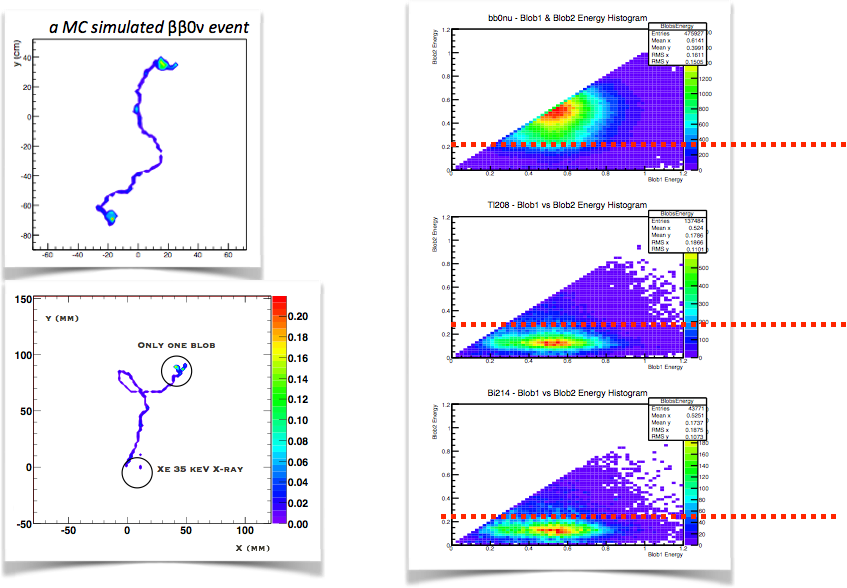
\includegraphics[width=0.9\textwidth]{img/Topology.png}
\caption{\small NEXT has a topological signature, not available in most \bbonu\ detectors. The panel shows the reconstruction of a Monte Carlo signal (topleft) and background (bottomleft) event. The signal has two electrons (two blobs). The background has only one electron (one blob) and the associated emission of a 35 keV X-ray. The color codes energy deposition in the TPC. An scatter plot of the energy of the two blobs shows a clear separation between signal and background regions.}\label{fig.ETRK2}
\end{figure}
%%%%%

%%%%%
\begin{figure}
\centering
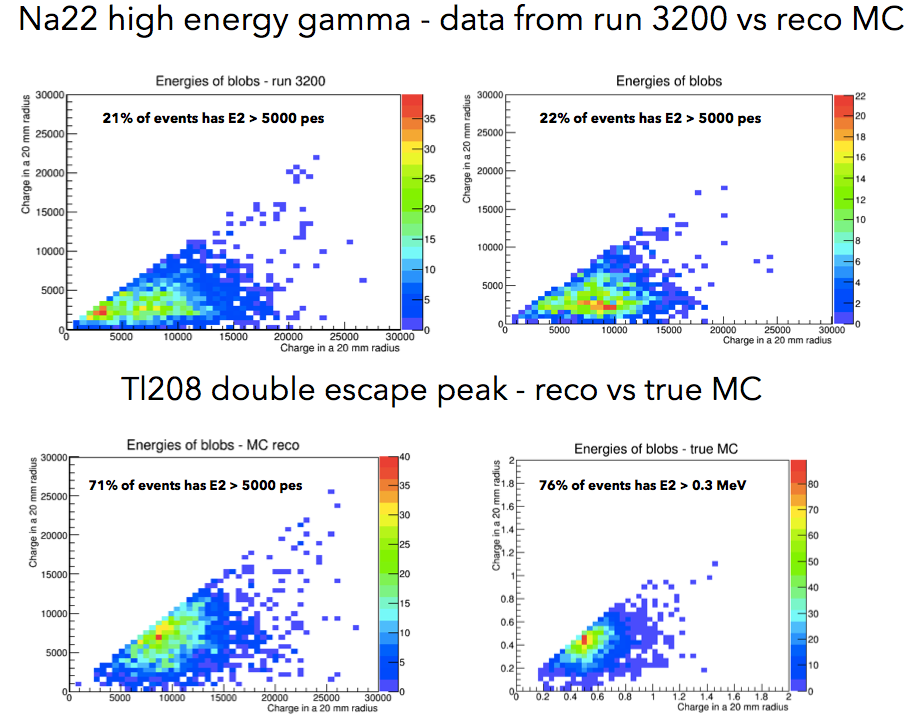
\includegraphics[width=0.9\textwidth]{img/ElectronsDataMC.png}
\caption{\small A comparison between data (left) and Monte Carlo (right) for electrons of different energies recorded in the DEMO chambers, showing the very good agreement between both data sets and therefore the robustness of the topological signal, unique of the NEXT experiment.}\label{fig.ETRK3}
\end{figure}


Double beta decay events leave a distinctive topological signature in HPXe: a continuous track with larger energy depositions (\emph{blobs}) at both ends due to the Bragg-like peaks in the d$E$/d$x$ of the stopping electrons (figure \ref{fig.ETRK2}, topleft). In contrast, background electrons are produced by Compton or photoelectric interactions, and are characterised by a single blob and, often, by a satellite cluster corresponding to the emission of $\sim30$-keV fluorescence x-rays by xenon (figure \ref{fig.ETRK2}, bottomleft).
Reconstruction of this topology using the tracking plane provides a powerful means of background rejection, as can be observed in the figure. In our TDR we chose a conservative cut to separate double--blob from single--blob events which provided a suppression factor of 20 for the background while keeping 80\% of the signal.  DEMO has reconstructed single electrons from \NA\ and \CS\ sources, as well as double electrons from the double escape peak of \TL\, demonstrating the robustness of the topological signal. 

%
Figure \ref{fig.ETRK3} shows a comparison between data and Monte Carlo for electrons interacting in the DEMO detector. Two radioactive sources were used: Na-22, producing single electrons of 511 keV, and Tl-208, whose double escape peak produced {\em double electrons}, at the energy of 1.6 MeV. Both data sets allow us to ``mimic'' signal and background and thus have a robust assessment of the performance of the topological signal comparing the Monte Carlo simulation and the actual results obtained with DEMO. The agreement between both data sets is very good, revealing the robustness of the topological signal. 

\subsection{Energy resolution}

%%%%%
\begin{figure}
\centering
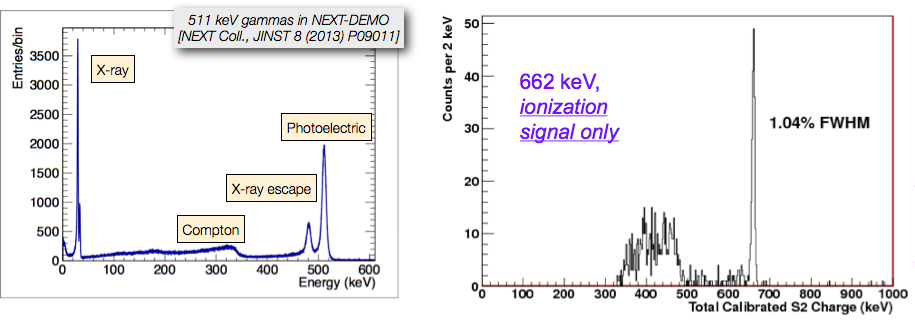
\includegraphics[width=0.9\textwidth]{img/EResolution.png}
\caption{\small Left: the full energy spectrum measured for electrons of 511 keV in the DEMO detector. Right the spectrum near the photoelectric peak for 662 keV electrons in NEXT-DBDM. The resolution at 662 keV is 1\% FWHM (0.5\% FWHM at \Qbb). The resolution extrapolated from 511 keV is 0.7\%.}\label{fig.ERES}. 
\end{figure}
%%%%

Figure \ref{fig.ERES} shows the resolution obtained with the NEXT-DBDM apparatus. A resolution of 1\% FWHM with 
662 keV photons, has been measured, which extrapolates to 0.5\% FWHM at \Qbb. This result is not far from the expected limit obtained adding in quadrature the different factors that contribute to the resolution (Fano factor, photoelectron statistics and electronic noise). The resolution measured in NEXT-DEMO extrapolates to 0.7\% FWHM. The difference between both prototypes is due to better photoelectron statistics and aspect ratio in DBDM. The results, are, in any case, better than the target of 1\% FWHM described in the TDR.

The status of the NEXT experiment and the results achieved by the prototypes have been described in a recent
paper \footcite{Gomez-Cadenas:2013lta}.


\subsection{\label{sec.new}The NEW detector.}

%%%%%%%%%%
\begin{figure}
\centering
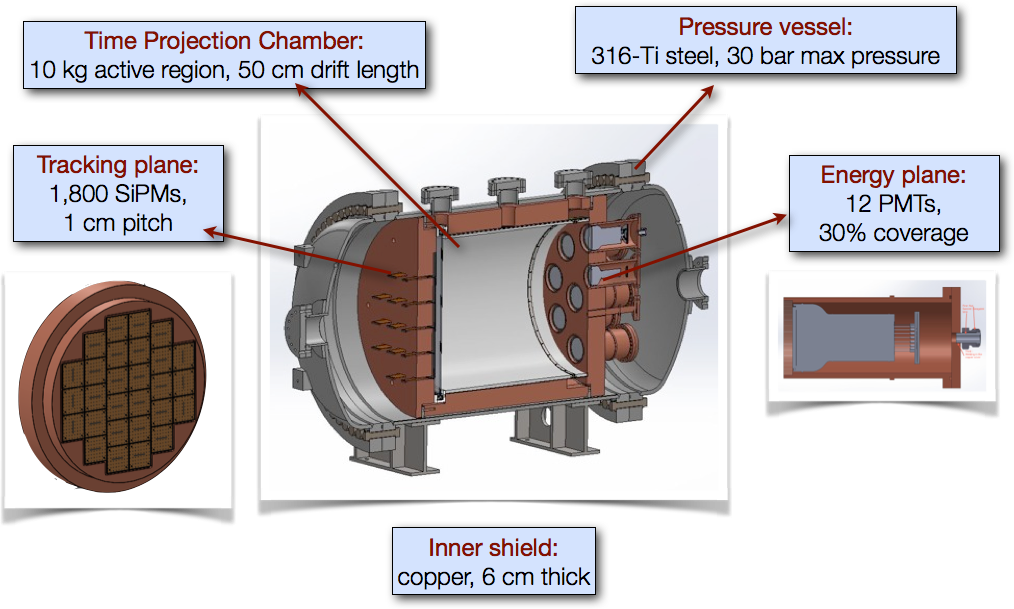
\includegraphics[height=9cm]{img/NEW.png}
\caption{\small The NEW apparatus.} \label{fig:NEW}
\end{figure} 

The NEW (NEXT-WHITE) apparatus\footnote{The name honours the memory of the late Professor James White, one of the key scientists of the NEXT Collaboration.}, shown in Figure \ref{fig:NEW}, is the first phase of the NEXT detector to operate underground. NEW 
%has a triple goal:
%
%\begin{enumerate}
%\item {\bf Technology}: it will validate the technological solutions adopted by NEXT-100.
%\item {\bf Radiopurity}: it will allow the NEXT collaboration an extra step in the implementation of a radiopure detector.
%\item {\bf Physics}: it will demonstrate with measurements of the \BI\ and \TL\ lines, as well as with the measurement of the \bbtnu\ spectrum, the physics capabilities of NEXT-100.
%\end{enumerate}
%
is a scale 1:2 in size (1:8 in mass) of NEXT-100. The energy plane contains 12 PMTs (20 \% of the 60 PMTs deployed in NEXT-100). The tracking plane technology consists of 30 Kapton Dice Boards (KDB) deploying 1800 SiPMs (also 20\% of the sensors). The field cage has a diameter of 50~cm and a length of 60~cm (the dimensions of the NEXT-100 field cage are roughly 1~m long and 1.2~m diameter). 

NEW is a necessary step\footnote{As formally stated by the scientific committee of the LSC, who recommended its construction in 2013.} towards the construction of NEXT-100. It will validate the technological solutions adopted by the collaboration and, as discussed below, it is essential in the definition of the project methodology. Furthermore, The NEXT background model is currently based on a sophisticated Monte Carlo simulation of all expected background sources in each part of the detector. NEW will allow the validation of the background model with actual data. 
%Last but not least, NEW operation will demonstrate with measurements of the \BI\ and \TL\ lines, as well as with the measurement of the \bbtnu\ spectrum, the physics capabilities of NEXT-100.

Furthermore, the calibration of NEW with 
sources of higher energy, will allow a precise study of the evolution of the resolution with the energy. 
In particular it will be plausible to measure the resolution near \Qbb\ using a Thorium source, which provides 2.6 MeV gammas. Last, but not least, we intend to 
reconstruct the spectrum of \bbtnu. Those events are topologically identical to signal events (\bbonu) and can be used to demonstrate with data the power of the topological signature. 
%

\subsection{Discovery potential of NEXT-100.}

The excellent resolution of NEXT (0.5 \% FWHM), and the combination of a low radioactive budget with a topological signature (which yields an expected background rate of $5 \times 10^{-4} \ckky$), will allow the NEXT-100 detector to reach a sensitivity to the \bbonu\ period of $\Tonu > 7 \times 10^{25}$~yr for a exposure of 300 kg$\cdot$yr. This translates into a \mbb\ sensitivity range as low as $[67-187]$~meV, depending on the NME. Therefore NEXT-100 will have a substantial chance of making a discovery if the NME is sufficiently high (see Fig.~\ref{fig.mbb}). 

\section{Towards a ton-scale high-pressure xenon TPC.}

%%%%%%
\begin{figure}
\centering
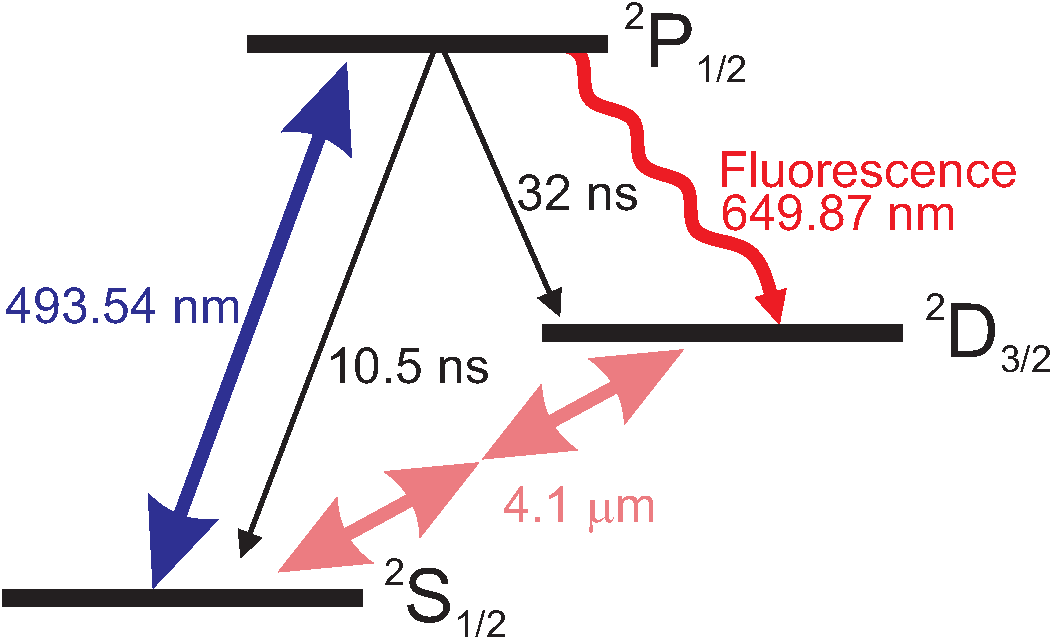
\includegraphics[width=0.60\textwidth]{img/levelscheme2.pdf}
\caption{\small The \BATA\ concept.} \label{fig.BATA}
\end{figure}
%%%%%%

If no discovery is made by the current generation of experiments, the full exploration of the CRR region (corresponding to the inverted hierarchy of neutrino masses, and \mbb\ values as low as 15~meV) requires detectors of larger mass (at least 1 ton), good resolution and extremely low specific background. The \HPXE\ technology has the potential to provide the most sensitive detector at this scale, by scaling the detector to a mass in the range of one ton and adding additional handles to further suppress the background. 

\subsection{Barium Tagging}

One of the most promising possibilities is to develop the technology to unambiguously tag the barium ion produced in the xenon decay, $Xe \rightarrow Ba^{++} + 2 e^-$. The conceptual idea to tag $Ba^{+}$ is illustrated in Figure \ref{fig.BATA}. A ``blue'' laser of wavelength 493.54 nm excites (``pumps'') the S state, inducing $S \rightarrow P$~transitions, with a lifetime of $\sim$ 10 ns. About 30 \% of the times the \TwoP\ states decay to the state \TwoD, emitting ``red'' (649.76 nm) fluorescence in a characteristic time of 30 ns. The state \TwoD\ is metastable, but a second laser of suitable wavelength (4.1 $\mu$m) can be used to induce the transition to the ground state (this is known as ``deshelving'').  The whole cycle takes less than 50 ns, and therefore several millions of red fluorescence photons can be emitted by a single ion. 

The practical application of this conceptual idea is by no means easy, and in fact, it has been shown to be extremely difficult in liquid xenon by the work of the EXO collaboration\footcite{Dolinski:2012dta}. However, it may be feasible in a \HPXE\ detector, where a number of fortunate conditions may occur. These conditions are: a) charge reduction of the emitted barium ion, from $Ba^{++}$~to $Ba^{+}$, which can be induced by collisions with xenon atoms, or by the addition of a suitable quencher; b) ``trapping'' of the barium ion ``in situ'' by the surrounding Xe atoms, which result in a very low drift velocity for the ion; c) location of the ion, via the reconstruction of the event topology. 

All the above needs to be demonstrated with a systematic R\&D program, which must also address additional experimental issues such as pressure broadening of the laser, filtering of Rayleigh scattering, and others. The EXO collaboration has carried out extensive research of the potential for Barium Tagging, not only in a LXe TPC, but also in an \HPXE, where promising results are obtained\footnote{See for example, {\em MOBILITY AND FLUORESCENCE OF BARIUM IONS IN XENON GAS FOR THE EXO EXPERIMENT},
Ph.D. thesis, Julio Cesar Benitez Medina, Department of Physics
Colorado State University,
Spring 2014.}. NEXT, on the other hand, has started a collaboration with CLPU\footcite{clpu}, a Spanish national facility dedicated to ultra-intense lasers, with the aim of carrying out a systematic R\&D program to understand the potential of Barium Tagging in a high pressure gas xenon TPC. We believe that such a program offers also a unique opportunity of joint development with the EXO collaboration. Clearly the construction of a ton-scale \HPXE\ detector implementing the full Barium Tagging technology is a very challenging enterprise. On the other hand, it appears to be a promising path towards the future. 


\subsection{Adding a magnetic field to enhance the topological signal}

%%%%%%%
\begin{figure}
\centering
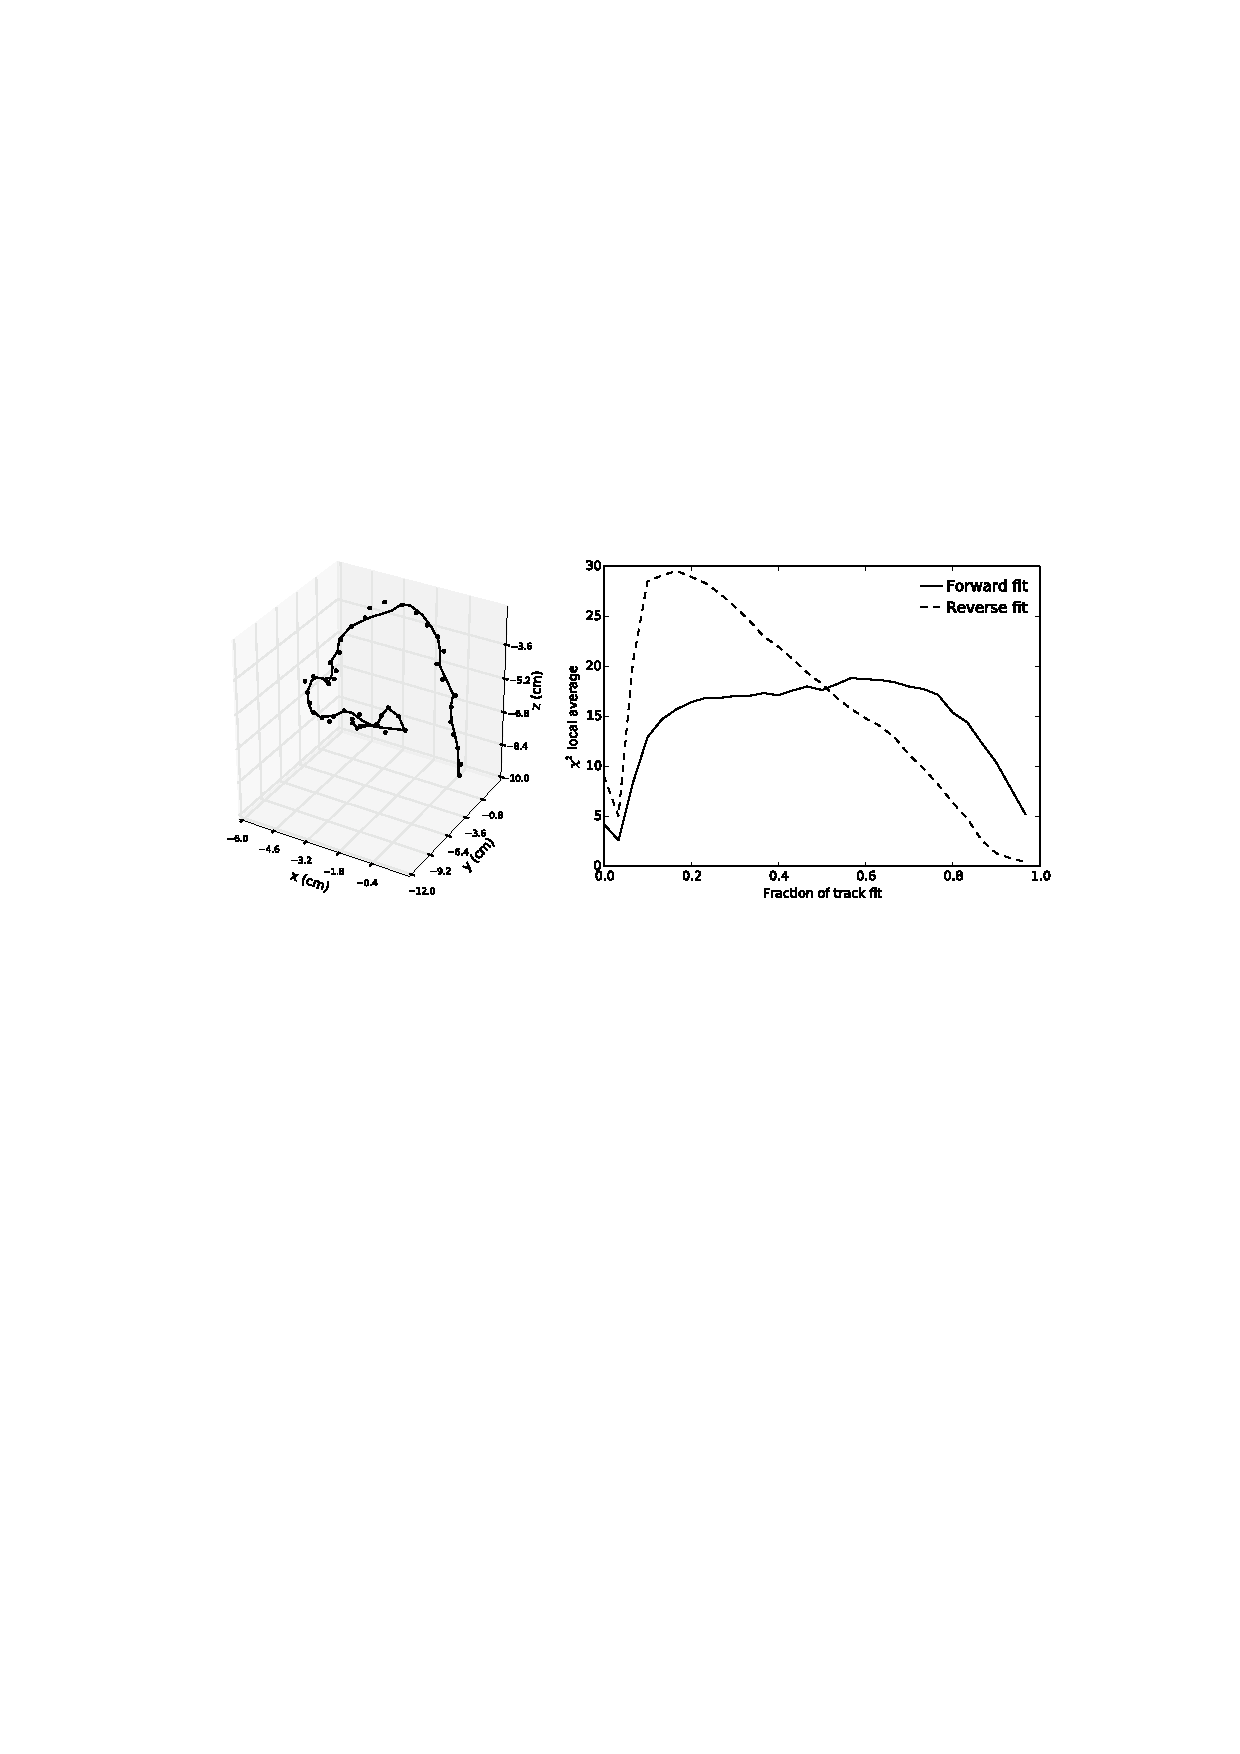
\includegraphics[width=0.99\textwidth]{img/KALMAN.pdf}
\caption{\small A Kalman Filter fit to a simulated (1 mm resolution) single-electron track in the proper direction of momentum flow. (Right) The local $\chi^2$ values produced along different points of the proper (“forward”) and improper (“reverse”) fits, averaged over $10^4$ single-electron tracks. Since the initial momentum is assumed to be the same in both fits, the $\chi^2$ value is artificially high at the beginning of the reverse fit (low multiple scattering error assumed, high multiple scattering found) and artificially low at the end (high multiple scattering error assumed, low multiple scattering found) .} \label{fig.KF}
\end{figure}
%%%%%%

On the other hand, we believe that there are further ways to improve the \HPXE\ technology in addition to Barium Tagging. Specifically, we believe that the addition of a moderate magnetic field will improve the NEXT rejection background by as much as an order of magnitude. 

In the presence of a uniform external magnetic field B, both of the emitted electrons in a $\bbonu$ (or a $\bbtnu$) decay, should spiral around the field lines in circular motion with radius $r = p_T/eB$, where $p_T$~ is the momentum of the electron transverse to the direction of the field and $e$~ is the electron charge. A single energetic electron should produce a clear single spiral with radius indicative of its momentum, and a double-electron track with the same energy will produce two spirals each with much less momentum. This information provides an additional way of separating single-electrons arising from background processes from double electrons produced in \bb\ decays, {\bf in spite of the large multiple scattering that the electrons suffer in a dense \HPXE}.

Multiple scattering occurs as an energetic electron traverses a dense medium --it undergoes several large-angle scatters that sharply divert an otherwise relatively smooth path through the detector, and the variance on angle of these scatters becomes larger at lower momentum--. On the other hand, using the mathematical technique known as the Kalman Filter\footcite{Cervera:2002} and incorporating multiple scattering as a noise process, fits to reconstructed electron tracks in both directions, {\bf assuming they are single-electron tracks with initial momentum corresponding to the kinetic energy released in $\bbonu$},  give different results for single and double-electron tracks, as illustrated in Figure \ref{fig.KF}. For single-electron tracks, the fit should perform well in one direction (from the production vertex to the end vertex, since in this case the fit hypothesis is correct) and poorly in the other direction (from end vertex to production vertex, since now the hypothesis is totally wrong, and the electron has, as the start of the fit, vanishing momentum). For double-electron tracks, the fit should fail in both directions. 

The illustrative result displayed in Figure \ref{fig.KF}\footnote{J.J. Gomez-Cadenas, J. Renner, A. Cervera, J.A. Hernando, A. Imzaylov, F. Monrabal and J. Muñoz, ``Enhancing the topological signature of an HPXe detector by means of a magnetic field'', in preparation.} shows how the ``forward fit'' (from production to end vertex), differs from the ``reverse fit'' (from end vertex to production vertex''), {\em even in the absence of a magnetic field}.  The right panel of the figure displays the local $\chi^2$~at each step of the fit. In the case of the forward fit (correct hypothesis), the fit converges rapidly to a flat value, since the Kalman Filter keeps updating the momentum o the electron as it losses energy by ionisation. Since the Kalman Filter model incorporates multiple scattering, the trajectory of the electron can indeed be tracked, as shown in the left panel of the figure. Instead, the local $\chi^2$~for the reverse fit is too high at the beginning of the fit (the hypothesis is that the momentum is large, when in fact is is very small, therefore the predicted multiple scattering error is underestimated) and too small at the end of the fit (where the situation is reversed and thus the predicted multiple scattering error is overestimated).  

In the simulation, the assumed point-error is 1 mm. Such a resolution is difficult to achieve in NEXT-100, unless some additive to reduce the transverse diffusion is added. However, when a solenoidal magnetic field is added the E$\times$B effect reduces the lateral diffusion to negligible levels for any reasonable value of the field ($B=0.1$~Tesla is used for the simulations). In NEXT-100, position is reconstructed using SiPMs spaced at a pitch of 10 mm, yielding a resolution (if one would not make use of the SiPM recorded charge to weight the event position) of 3 mm, which improves to $\sim$~1 mm when the position is weighted by the SiPM recorded charge. Therefore, the resolution assumed in the plot is correct in the presence of a magnetic field (it could also be achieved adding suitable additives such as TMA). 

To further enhance the topological signature of NEXT (see Figure \ref{fig.ETRK2}), one performs a Kalman Fit to double-electron candidates (that is, those which have passed the selection cut requiring that the energy of the two blobs defining the beginning and end of the track is large). As noted, in true signal events, the momentum in each blob vanishes (each blob corresponds to the end-vertex of one of the two electrons emitted in a \bb\ decay). In background events managing to ``fake'' a blob at the start of the track, the fit will succeed in one direction (when we start from the fake blob, in which case the momentum is 2.3 MeV, corresponding to the kinetic energy of \Qbb), and will fail in the other (when we start from the true blob, where the momentum vanishes). Thus, fitting the candidates surviving the standard topological cut of NEXT, {\em under the hypothesis that they are background electrons}, provide an extra rejection criteria for background. We fit the trajectory of the electron starting from both ends, and accept it only if the fit is consistent, in both cases, with a reverse fit.  This simple approach yields a factor 5 extra rejection (for 90\% signal efficiency), {\em in the absence of a magnetic field}.

Indeed, the rejection in the absence of magnetic field comes from an {\em indirect} measurement of the momentum of the electrons through their multiple scattering
angle $\theta_0$:

\begin{equation}
\theta_{0} = \frac{13.6}{\beta c p}\sqrt{\frac{x}{X_0}}+(1 + 0.038 \log{\frac{x}{X_0}})
\end{equation}
% 
 where $X_0$ is the radiation length of the dense xenon gas 
 $\sim P \times 8.48 ~g\cdot cm^{-2}$~where $P$~is the pressure of the gas) 
 $\beta c$~is the velocity of the electron and $p$~its momentum. 
 
 When a magnetic field $B$~ is added the (transverse) momentum of the electrons can be 
 directly measured,  $p_T = r \times B$. The determination of $p_T$ does not need to be accurate (which is fortunate, given the fact that the trajectory of the electrons is smeared by multiple scattering), because one applies the strategy described above. Single (background) electrons will yield a good forward fit (where now the momentum of the electron must be consisted with the track curvature) and a bad reverse fit. Double (signal) electrons will yield reverse fits in two directions. Indeed, for candidate signal (double) electrons is is possible to scan the starting point of the reverse fit in both directions, until a good forward fit is found. This corresponds to the vertex of the double electron. 
 
 Work is in progress to assess the final rejection factor and efficiency obtained when a magnetic field is added (the range of the magnetic field for pressures between 10-20 bar appears to be $\sim$0.1 Tesla) and both topological signatures (blob and vertex signatures) are combined, but our preliminary studies indicate that adding the vertex signature will provide a factor of 10 extra rejection of backgrounds at little cost (90\%) to the signal efficiency.  
 
 The current (estimated) rejection factor for NEXT-100 is 0.4 counts per ton and keV in a year. If a resolution of \Qbb\ of 0.5 \% FWHM is confirmed in the large detector as we expect, this translates into 5 counts per ton in the ROI. The addition of a magnetic field may yield a value of 0.5-1 counts per ton in the ROI, thus allowing the HPXe technology to operate in the ton regime without being background limited. 
  
\subsection{NEXT will be BEXT}
The addition of either a B-field or Barium Tagging (or both), are clear forward paths to improve the NEXT detector towards the future BEXT\footnote{B-field Experiment with a Xenon TPC, also Barium-Taggin Experiment with a Xenon TPC} apparatus, displaying  
a mass in the range of several tons, with a resolution of 0.5 \% FWHM and a background rate in the range of $10^{-4}$ (this appears relatively easy to achieve with a magnetic field) to $10^{-6}$ (as ultimately possible with barium-tagging) \ckky\ would be able to fully cover the CRR (and inverted hierarchy) region event in the most pessimistic NME scenario. 



